\chapter{Dataset}
\label{chap:tap_du_lieu}
	\textit{Trong chương này, chúng tôi giới thiệu tập dữ liệu 3D-IRCADb-01 mà chúng tôi đã sử dụng để đánh giá hệ thống. Sau đó, chúng tôi trình bày các vấn đề cần xử lý đối với tập dữ liệu này trước khi có thể sử dụng.}
\minitoc

\section{Giới thiệu chung}
\label{sec:gioi_thieu_chung}
	\begin{figure}[h!]
		\centering
		
\includegraphics[width=.4\textwidth]{figures/ircad_logo}
		\caption{Logo Viện nghiên cứu chống ung thư đường tiêu hoá ở Pháp.}
		\sourcefig{\url{https://www.ircad.fr}.}
		\label{fig:3d_ircadb_01_visualize}
	\end{figure}
	\textit{3D-IRCADb} (3D Image Reconstruction for Comparison of Algorithm Database) là tập dữ liệu do Viện nghiên cứu chống ung thư đường tiêu hoá \textit{IRCAD} cung cấp và là tập dữ liệu đáp ứng tốt nhất cho bài toán trong đề tài của chúng tôi. Tập dữ liệu này cung cấp một số bộ ảnh y khoa từ các bệnh nhân được ẩn danh. Với mỗi bộ ảnh, các cơ quan, cấu trúc khác nhau được phân đoạn thủ công bởi các chuyên gia lâm sàng.
	
	\textit{3D-IRCADb} có hai gói dữ liệu là \textit{3D-IRCADb-01} và \textit{3D-IRCADb-02}. Chúng tôi chọn sử dụng gói \textit{3D-IRCADb-01} \cite{3D-IRCADb-01} để đánh giá hệ thống trong luận văn này. \textit{3D-IRCADb-01} bao gồm ảnh CT của 20 bệnh nhân (10 nam và 10 nữ) với sự xuất hiện của khối u gan trong 75\% các trường hợp. Hệ thống mạch máu trong các bộ ảnh CT được chia thành ba phần là tĩnh mạch chủ, tĩnh mạch cửa và động mạch và được phân đoạn riêng cho từng loại mạch máu. \autoref{fig:3d_ircadb_01_visualize} là ảnh trực quan dữ liệu cho từng bệnh nhân trong gói \textit{3D-IRCADb-01}. Các thông số chi tiết về gói dữ liệu này được chúng tôi trình bày trong \autoref{appendix:thong_so_tap_du_lieu_3d_ircadb_01}.
	\vfill
	\begin{figure}[h!]
		\centering
		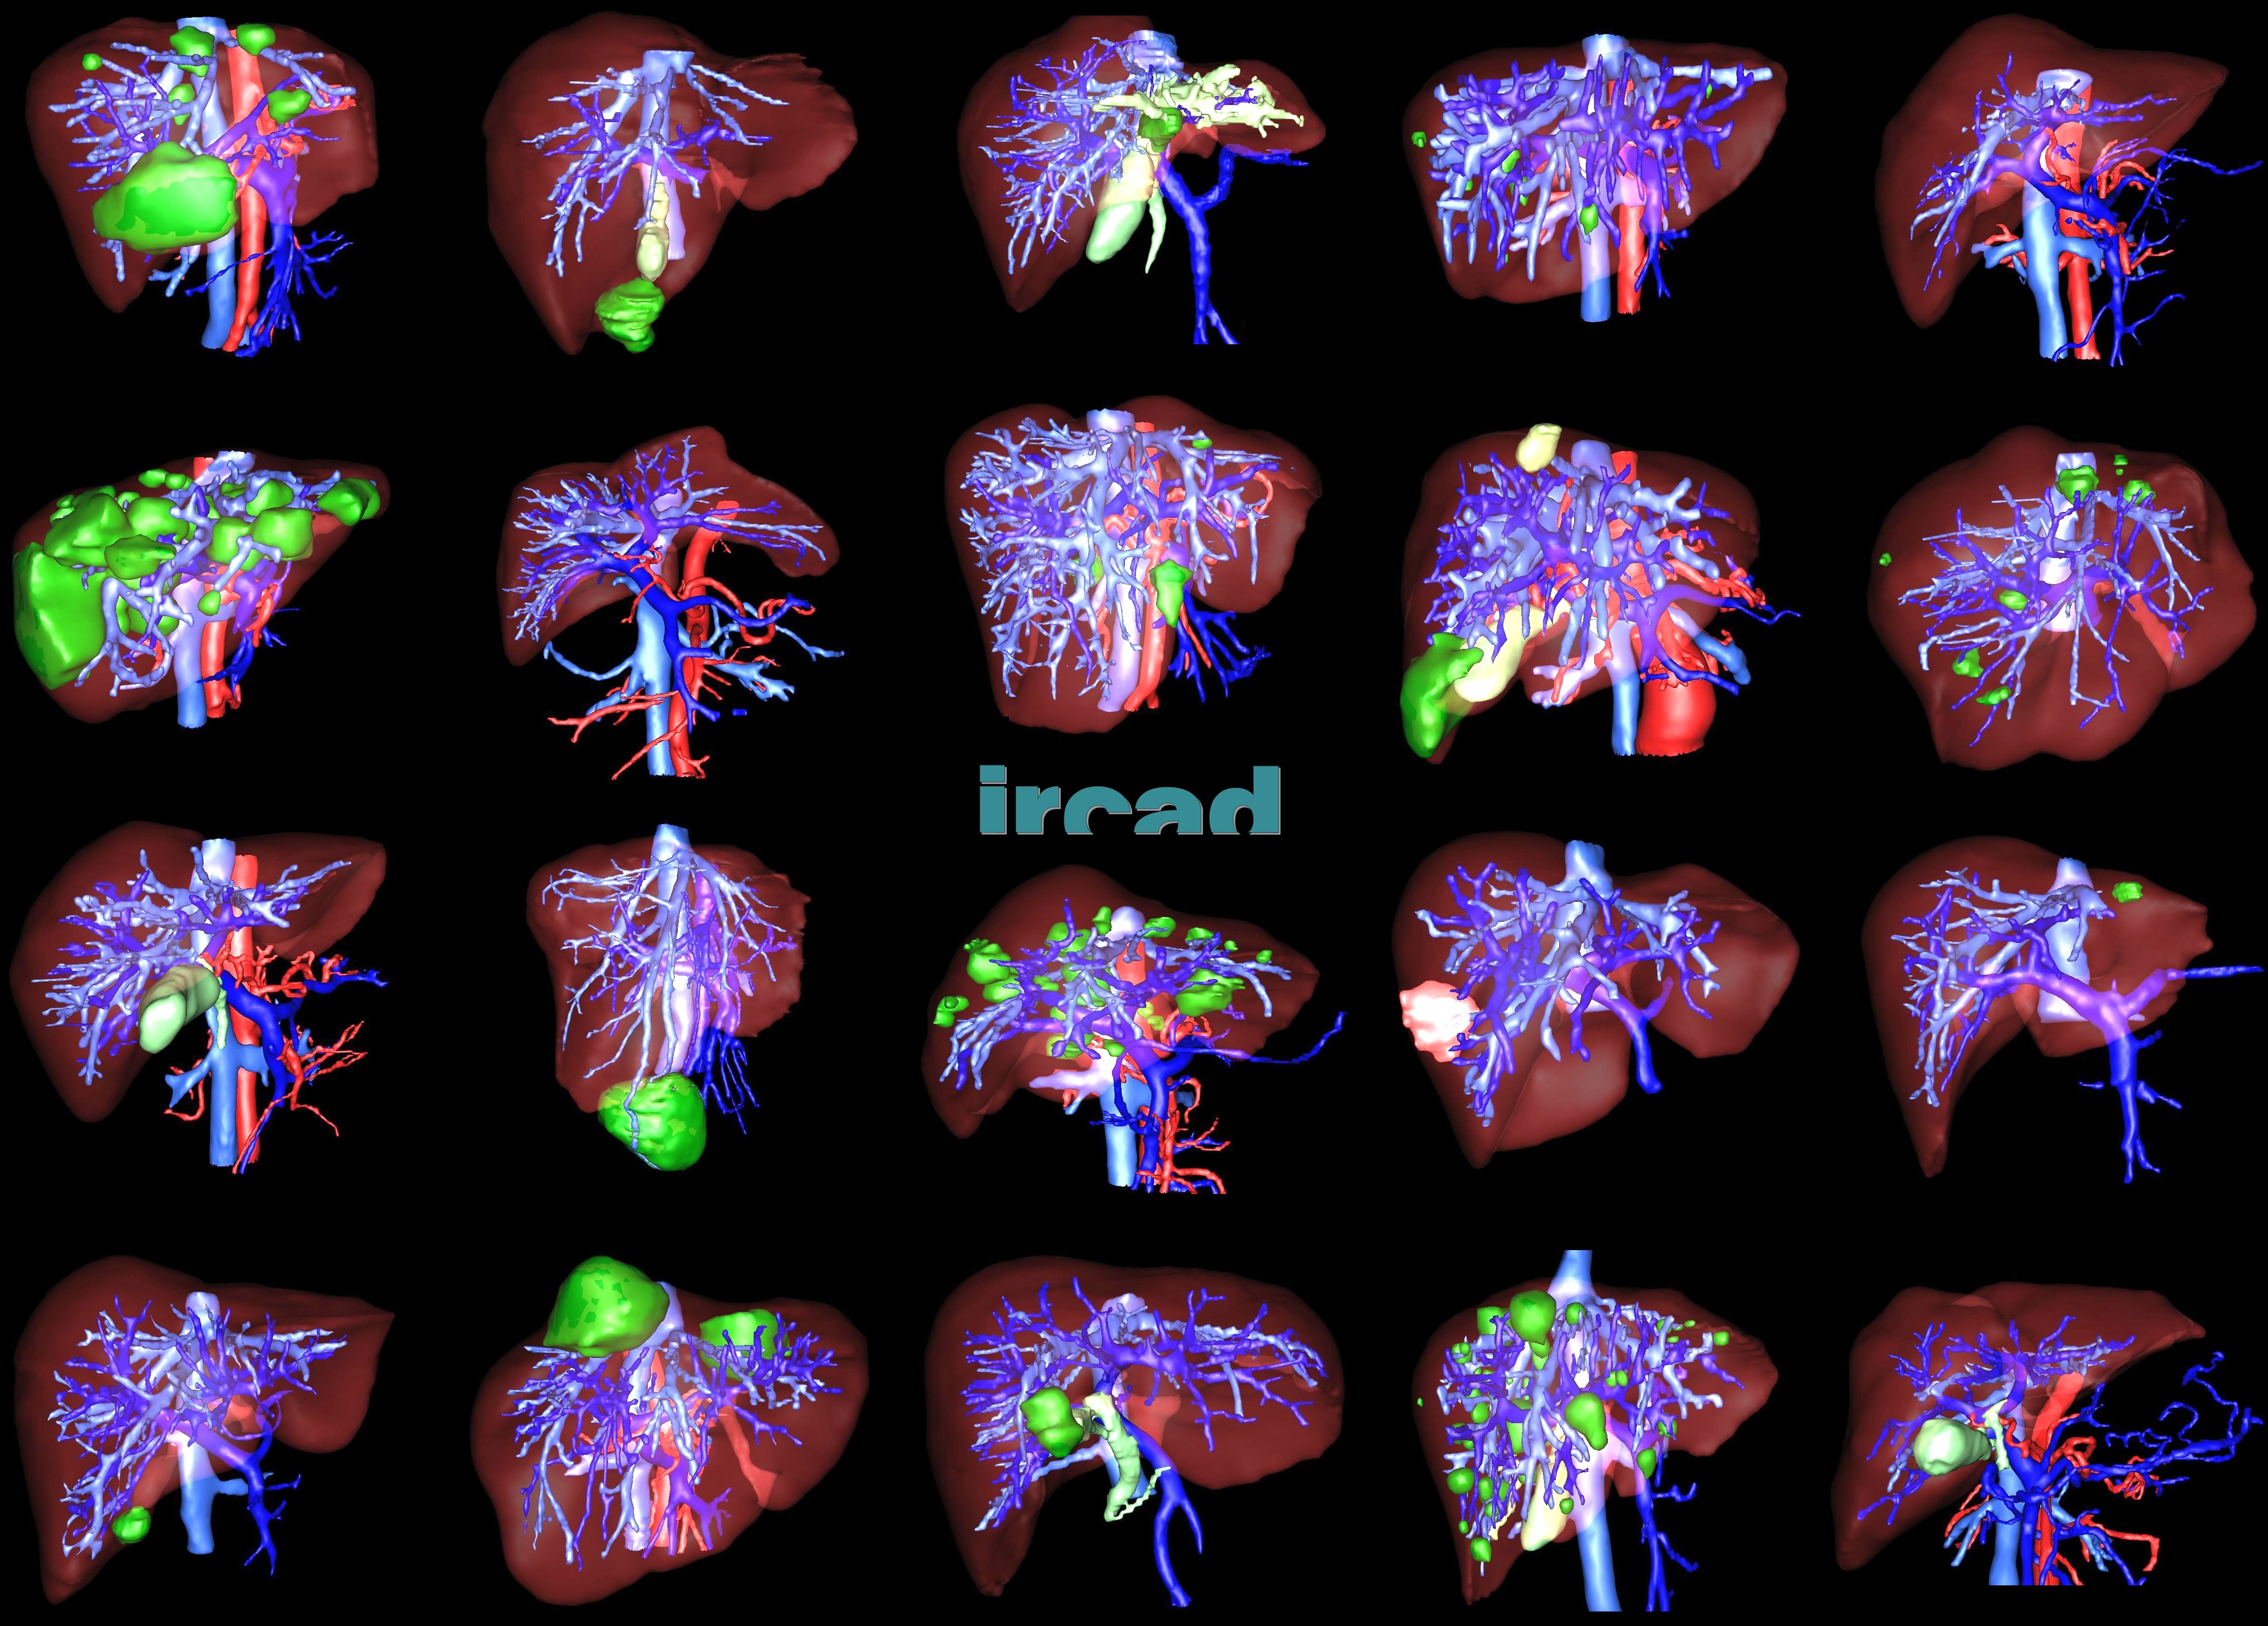
\includegraphics[width=\textwidth, height=.672\textwidth]{figures/ircad_dataset}
		\caption[Ảnh trực quan gói dữ liệu \textit{3D-IRCADb-01}.]{Ảnh trực quan gói dữ liệu \textit{3D-IRCADb-01} \sourcefig{\cite{3D-IRCADb-01}}.}
		\label{fig:3d_ircadb_01_visualize}
	\end{figure}

\section{Các vấn đề cần xử lý}
\label{sec:cac_van_de_can_xu_ly}
	Trong mục này, chúng tôi trình bày các vấn đề gặp phải đối với tập dữ liệu cần được chú ý và (hoặc) xử lý trước khi có thể sử dụng bao gồm đơn vị hounsfield, nhãn phân đoạn không đầy đủ và giá trị nhãn không nhất quán.
	
\subsection{Đơn vị Hounsfield}
\label{subsec:don_vi_hounsfield}
	Nếu trong khoa học máy tính giá trị của một điểm ảnh được đo bằng cường độ sáng (intensity\index{Intensity}), thì trong y khoa giá trị của một điểm ảnh trên ảnh CT được đo bằng đơn vị hounsfield\index{Hounsfield} (xem \cite{medicalconnections}). Cách tính giá trị hounsfield như sau
	\begin{equation}
		HU = m * P + b,
		\label{eqn:hounsfield}
	\end{equation}
	trong đó, $HU$ là giá trị hounsfield, $P$ là giá trị số của điểm ảnh, $m$ là giá trị tại trường (0028,1053) ``Rescale slope'' và $b$ là giá trị tại trường (0028,1052) ``Rescale intercept'' được lưu trong file DICOM\footnote{DICOM là định dạng chuyên dụng cho ảnh CT.}. Đối với bộ dữ liệu \textit{3D-IRCADb-01}, $m$ và $b$ đều có giá trị là 1 nên ta có thể sử dụng trực tiếp không phải thực hiện bước tính giá trị hounsfield.
	
\subsection{Nhãn phân đoạn không đầy đủ}
\label{subsec:nhan_phan_doan_khong_day_du}
	Trong đề tài này, chúng tôi quan tâm các thành phần trong tập dữ liệu liên quan đến cơ quan gan và hệ thống mạch máu. Tuy nhiên, sau khi khảo sát tình trạng của tập dữ liệu, chúng tôi phát hiện tập dữ liệu có hai vấn đề về tính đầy đủ của nhãn phân đoạn.
	
	\textbf{Thứ nhất,} nhãn phân đoạn không đầy đủ cho các loại mạch máu. Khi tìm kiếm các tệp tin liên quan đến hệ thống mạch máu trong tập dữ liệu, chúng tôi phát hiện có rất nhiều bệnh nhân không có nhãn phân đoạn cho động mạch.
	
	\textbf{Thứ hai,} nhãn phân đoạn không đầy đủ trên tất cả các lớp ảnh. \autoref{fig:miss_label_patient_2} là ví dụ về việc gán nhãn không đầy đủ trên các lớp ảnh cho tĩnh mạch ở bệnh nhân số 2. \autoref{fig:miss_label_patient_2_dicom_74} và \autoref{fig:miss_label_patient_2_mask_74} lần lượt là lớp ảnh CT thứ 74 chứa tĩnh mạch và nhãn phân đoạn tương ứng bị gán thiếu. Trong khi \autoref{fig:miss_label_patient_2_dicom_75} là lớp ảnh CT liền kề với nhãn phân đoạn tĩnh mạch đầy đủ như \autoref{fig:miss_label_patient_2_mask_75}.
	
	\autoref{tab:3d_ircadb_01_state} tổng hợp tình trạng nhãn phân đoạn của cơ quan gan và hệ thống mạch máu bao gồm tĩnh mạch chủ, tĩnh mạch cửa và động mạch. Ở mỗi đối tượng, bảng cho biết nhãn phân đoạn tương ứng có được cung cấp hay không và những lớp ảnh nào trong tổng số các lớp ảnh được gán nhãn.
	\newpage\null\vfill
	\begin{figure}[h!]
		\begin{subfigure}[b]{0.475\textwidth}
			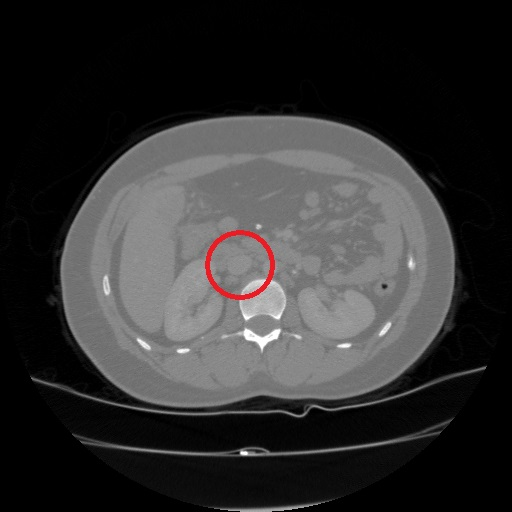
\includegraphics[width=\textwidth]{figures/miss_label_patient_2_dicom_74}
			\caption{}
			\label{fig:miss_label_patient_2_dicom_74}
		\end{subfigure}
		\hfill
		\begin{subfigure}[b]{0.475\textwidth}
			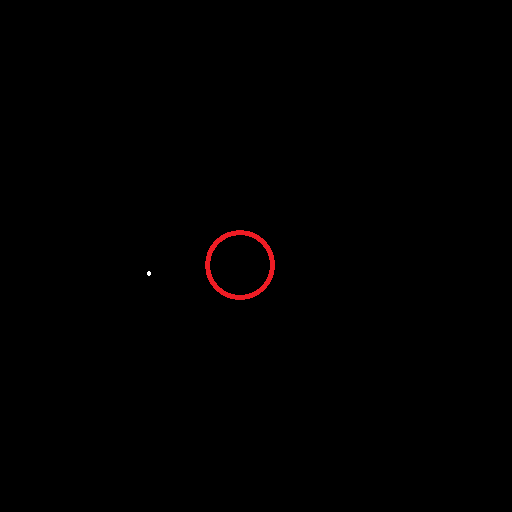
\includegraphics[width=\textwidth]{figures/miss_label_patient_2_mask_74}
			\caption{}
			\label{fig:miss_label_patient_2_mask_74}
		\end{subfigure}\\[5mm]
		\begin{subfigure}[b]{0.475\textwidth}
			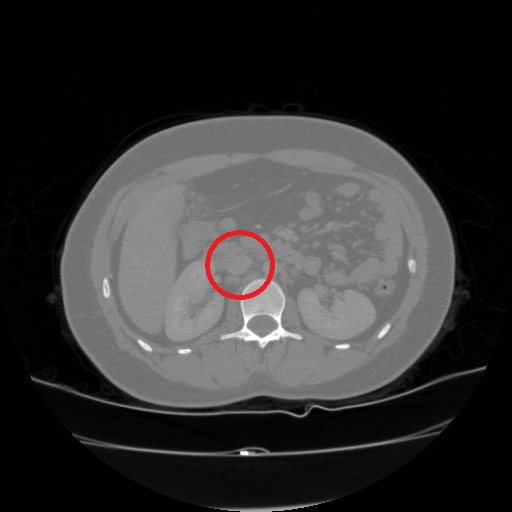
\includegraphics[width=\textwidth]{figures/miss_label_patient_2_dicom_75}
			\caption{}
			\label{fig:miss_label_patient_2_dicom_75}
		\end{subfigure}
		\hfill
		\begin{subfigure}[b]{0.475\textwidth}
			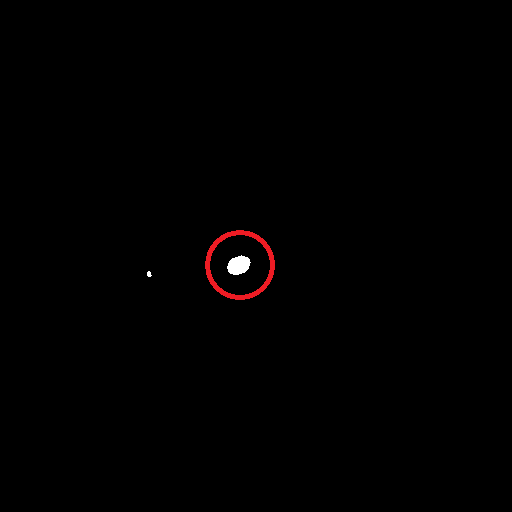
\includegraphics[width=\textwidth]{figures/miss_label_patient_2_mask_75}
			\caption{}
			\label{fig:miss_label_patient_2_mask_75}
		\end{subfigure}
		\caption[Nhãn phân đoạn bị thiếu trên một số lớp ảnh ở bệnh nhân số 2.]{Nhãn phân đoạn bị thiếu trên một số lớp ảnh ở bệnh nhân số 2. \subref{fig:miss_label_patient_2_dicom_74} ảnh CT lớp thứ 74 có tĩnh mạch chủ. \subref{fig:miss_label_patient_2_mask_74} nhãn phân đoạn cho ảnh CT lớp thứ 74 không được đánh nhãn tĩnh mạch chủ. \subref{fig:miss_label_patient_2_dicom_75} ảnh CT lớp thứ 75 có tĩnh mạch chủ. \subref{fig:miss_label_patient_2_mask_75} nhãn phân đoạn cho ảnh CT lớp thứ 75 được đánh nhãn tĩnh mạch chủ.}
		\label{fig:miss_label_patient_2}
	\end{figure}
	\vfill\newpage\null\vfill
	\begin{table}[h!]
		\newcommand\nextpatient{\\[2mm]}
		\centering
		\caption[Tình trạng nhãn phân đoạn của cơ quan gan và hệ thống mạch máu.]{Tình trạng nhãn phân đoạn của cơ quan gan và hệ thống mạch máu bao gồm tĩnh mạch chủ, tĩnh mạch cửa và động mạch. Kết quả khảo sát ở mỗi đối tượng cho biết nhãn phân đoạn của đối tượng đó có được cung cấp hay không và danh sách các lớp ảnh được~gán~nhãn.}
		\label{tab:3d_ircadb_01_state}
		\resizebox{\textwidth}{!}{%
			\begin{tabular}{cccccccccc}
				\toprule
				\multirow{2}{*}{\textbf{\begin{tabular}[c]{@{}c@{}}\\STT\\\end{tabular}}} & \multirow{2}{*}{\textbf{\begin{tabular}[c]{@{}c@{}}Số\\ lớp\\ ảnh\end{tabular}}} & \multicolumn{2}{c}{\textbf{Gan}} & \multicolumn{2}{c}{\textbf{Tĩnh mạch chủ}} & \multicolumn{2}{c}{\textbf{Tĩnh mạch cửa}} & \multicolumn{2}{c}{\textbf{Động mạch}} \\ \cmidrule{3-10} 
				&  & \textbf{\begin{tabular}[c]{@{}c@{}}Tồn\\ tại\end{tabular}} & \textbf{\begin{tabular}[c]{@{}c@{}}Được\\ gán nhãn\end{tabular}} & \textbf{\begin{tabular}[c]{@{}c@{}}Tồn\\ tại\end{tabular}} & \textbf{\begin{tabular}[c]{@{}c@{}}Được\\ gán nhãn\end{tabular}} & \textbf{\begin{tabular}[c]{@{}c@{}}Tồn\\ tại\end{tabular}} & \textbf{\begin{tabular}[c]{@{}c@{}}Được\\ gán nhãn\end{tabular}} & \textbf{\begin{tabular}[c]{@{}c@{}}Tồn\\ tại\end{tabular}} & \textbf{\begin{tabular}[c]{@{}c@{}}Được\\ gán nhãn\end{tabular}} \\ \midrule
				1 & 129 & Có & Đủ & Có & Đủ & Có & Đủ & Có & Đủ \nextpatient
				2 & 172 & Có & Đủ & Có & 75-152 & Có & 75-152 & Không & \_ \nextpatient
				3 & 200 & Có & Đủ & Có & 104-182 & Có & 104-182 & Không & \_ \nextpatient
				4 & 91 & Có & Đủ & Có & Đủ & Có & Đủ & Có & Đủ \nextpatient
				5 & 139 & Có & Đủ & Có & Đủ & Có & Đủ & Có & Đủ \nextpatient
				6 & 135 & Có & Đủ & Có & Đủ & Có & Đủ & Có & Đủ \nextpatient
				7 & 151 & Có & Đủ & Có & Đủ & Có & Đủ & Có & Đủ \nextpatient
				8 & 124 & Có & Đủ & Có & Đủ & Có & Đủ & Có & Đủ \nextpatient
				9 & 111 & Có & Đủ & Có & Đủ & Có & Đủ & Có & Đủ \nextpatient
				10 & 122 & Có & Đủ & Có & 49-113 & Có & 49-113 & Không & \_ \nextpatient
				11 & 132 & Có & Đủ & Có & Đủ & Có & Đủ & Có & Đủ \nextpatient
				12 & 260 & Có & Đủ & Có & 65-260 & Có & 65-260 & Có & 66-236 \nextpatient
				13 & 122 & Có & Đủ & Có & 1-117 & Có & 1-117 & Có & Đủ \nextpatient
				14 & 113 & Có & Đủ & Có & 51-113 & Có & 51-113 & Không & \_ \nextpatient
				15 & 125 & Có & Đủ & Có & 62-123 & Có & 62-123 & Không & \_ \nextpatient
				16 & 155 & Có & Đủ & Có & 32-143 & Có & 32-143 & Không & \_ \nextpatient
				17 & 119 & Có & Đủ & Có & Đủ & Có & Đủ & Có & Đủ \nextpatient
				18 & 74 & Có & Đủ & Có & 25-69 & Có & 25-69 & Không & \_ \nextpatient
				19 & 124 & Có & Đủ & Có & Đủ & Có & Đủ & Không & \_ \nextpatient
				20 & 225 & Có & Đủ & Có & Đủ & Có & Đủ & Có & Đủ \\ \bottomrule
			\end{tabular}
		}
	\end{table}
	\vfill\newpage
	
\subsection{Giá trị nhãn không nhất quán}
\label{subsec:gia_tri_nhan_khong_nhat_quan}
	Vấn đề tiếp theo của tập dữ liệu là giá trị nhãn phân đoạn không nhất quán. Đây là vấn đề nghiêm trọng mà nếu không xử lý trước khi sử dụng thì việc huấn luyện sẽ không thể thành công. 
	
	Trong hầu hết các nhãn phân đoạn có trong bộ dữ liệu, các giá trị background\index{Background} và foreground\index{Foreground} được gán số lần lượt là 0 và 255. Tuy nhiên, rất nhiều nhãn phân đoạn ở các cơ quan ở các bệnh nhân khác nhau được đánh giá trị khác nhau. \autoref{fig:label_value_patient_1} là ví dụ việc đọc lên khối nhãn phân đoạn tĩnh mạch chủ của bệnh nhân số 1 và in ra các giá trị riêng biệt, kết quả là tập giá trị chứa 0 và 255. Thực hiện thao tác tương tự trên bệnh nhân số 3, ta có kết quả là tập giá trị chứa 0 và 1 (\autoref{fig:label_value_patient_3}).
	\begin{figure}[h!]
		\begin{lstlisting}
path = "3Dircadb1/3Dircadb1.1/MASKS_DICOM/venoussystem/"

# Load all dicom files to numpy array.
volume = []
for i in range(len(os.listdir(path))):
	dicom = pydicom.dcmread(path + "image_" + str(i))
	volume.append(dicom.pixel_array)
volume = numpy.asarray(volume)

# Print unique value in volume.
numpy.unique(volume)
		\end{lstlisting}
		\hspace{7mm}\verb/array([  0, 255], dtype=uint8)/
		\caption{Giá trị nhãn phân đoạn tĩnh mạch chủ trên bệnh nhân số 1}
		\label{fig:label_value_patient_1}
	\end{figure}

	
	\begin{figure}[h!]
		\begin{lstlisting}
path = "3Dircadb1/3Dircadb1.3/MASKS_DICOM/venoussystem/"

# Load all dicom files to numpy array.
volume = []
for i in range(len(os.listdir(path))):
	dicom = pydicom.dcmread(path + "image_" + str(i))
	volume.append(dicom.pixel_array)
volume = numpy.asarray(volume)

# Print unique value in volume.
numpy.unique(volume)
		\end{lstlisting}
		\hspace{7mm}\verb/array([ 0, 1], dtype=uint8)/
		\caption{Giá trị nhãn phân đoạn tĩnh mạch chủ trên bệnh nhân số 3}
		\label{fig:label_value_patient_3}
	\end{figure}
	\newpage
	\autoref{tab:3d_ircadb_01_value} tổng hợp các giá trị background\index{Background} và foreground\index{Foreground} cho từng nhãn phân đoạn ở các cơ quan gan, tĩnh mạch chủ, tĩnh mạch cửa và động mạch. Từ đây, chúng tôi tiến hành chuẩn hoá giá trị nhãn phân đoạn về chung một bộ giá trị với background và foreground lần lượt là 0 và 1.

% Please add the following required packages to your document preamble:
% \usepackage{multirow}
\begin{table}[h!]
	\newcommand\nextpatient{\\[2mm]}
	\centering
	\caption{Giá trị nhãn phân đoạn của cơ quan gan và hệ thống mạch máu.}
	\label{tab:3d_ircadb_01_value}
	\begin{tabular}{ccccccccc}
		\toprule
		\multirow{2}{*}{\textbf{STT}} & \multicolumn{2}{c}{\textbf{Gan}} & \multicolumn{2}{c}{\textbf{Tĩnh mạch chủ}} & \multicolumn{2}{c}{\textbf{Tĩnh mạch cửa}} & \multicolumn{2}{c}{\textbf{Động mạch}} \\ \cmidrule{2-9} 
		& \textbf{BG\nomenclature{BG}{Background}} & \textbf{FG\nomenclature{FG}{Foreground}} & \textbf{BG} & \textbf{FG} & \textbf{BG} & \textbf{FG} & \textbf{BG} & \textbf{FG} \\ \midrule
		1 & 0 & 255 & 0 & 255 & 0 & 255 & 0 & 255 \nextpatient
		2 & 0 & 1 & 0 & 255 & 0 & 255 & \_ & \_ \nextpatient
		3 & 0 & 255 & 0 & 1 & 0 & 1 & \_ & \_ \nextpatient
		4 & 0 & 255 & 0 & 255 & 0 & 255 & 0 & 255 \nextpatient
		5 & 0 & 255 & 0 & 255 & 0 & 255 & 0 & 255 \nextpatient
		6 & 0 & 255 & 0 & 255 & 0 & 255 & 0 & 255 \nextpatient
		7 & 0 & 255 & 0 & 255 & 0 & 255 & 0 & 255 \nextpatient
		8 & 0 & 255 & 0 & 255 & 0 & 255 & 0 & 255 \nextpatient
		9 & 0 & 255 & 0 & 255 & 0 & 255 & 0 & 255 \nextpatient
		10 & 0 & 255 & 0 & 255 & 0 & 255 &\_  &\_  \nextpatient
		11 & 0 & 255 & 0 & 255 & 0 & 255 & 0 & 1, 255 \nextpatient
		12 & 0 & 1, 255 & 0 & 1 & 0 & 1 & 0 & 1 \nextpatient
		13 & 0 & 255 & 0 & 255 & 0 & 255 & 0 & 255 \nextpatient
		14 & 0 & 255 & 0 & 255 & 0 & 1, 255 &\_  &\_  \nextpatient
		15 & 0 & 255 & 0 & 255 & 0 & 255 & \_ & \_ \nextpatient
		16 & 0 & 255 & 0 & 255 & 0 & 255 & \_ & \_ \nextpatient
		17 & 0 & 255 & 0 & 255 & 0 & 255 & 0 & 255 \nextpatient
		18 & 0 & 1 & 0 & 255 & 0 & 255 & \_ &\_  \nextpatient
		19 & 0 & 255 & 0 & 255 & 0 & 255 & \_ &\_  \nextpatient
		20 & 0 & 1 & 0 & 1, 255 & 0 & 255 & 0 & 1, 255 \\ \bottomrule
	\end{tabular}
\end{table}
